\scanpage{24}\mspage{23}
b) $\Rightarrow$ a) Si $F'$ est un raffinement de $G$ tel que $F'$ sous figure de $F$, on a $|F|\subset|F'|\subset|G|$, et comme $|F|=|G|$ on
a $|F|=|F'|$, donc $F=F'$, puisque $F$ sous-figure de $F'$,
% slanted
\margin{\uline{Donnons aussi} condition équ\unsure{iv.|iv} c) \inserted{$F\ll G$ et} Toute strate de $G$ est réunion de strates de $F$. Et quand \unsure{on ne suppose plus|on ne suppose pas} \unsure{par avance|d'avance} que $F\ll G$, la condition d) \[\left\{\begin{aligned}&1^\circ)\ \text{Toute strate de }G\text{ est réunion de strates de }F\\&2^\circ)\ \forall \deleted{\unsure{B}}A\in F,\quad G^A=\{B\in G\mid B\supset A\}\text{ a un}\\&\text{plus petit élément.}\end{aligned}\right.\]}

a) $\Rightarrow$ b) Supposons que $|F|\ne|G|$, \deleted{soit $x\in|G|\setminus|F|$, considérons la} Il existe donc une figure $\deleted{F}H$ \deleted{qui soit} \inserted{telle} que \deleted{\unsure{vide}, qui soit un raffinement de $G$,}
\[ \left\{\begin{aligned} &|H|\ne\varnothing\\ &\deleted{F}H\ \text{raffine }G\\ &\deleted{F}H\ \text{disjointe de }F \end{aligned}\right. \]
par exemple on prend \unsure{un} $x\in|G|\setminus|F|$, et la figure $\deleted{F}H=\{\{x\}\}$. Or on a

\uline{Corollaire}\enspace Soient $F,H$ deux figures qui raffinent $G$, et telles que $F$ et $H$ \deleted{disjointes} \inserted{compatibles}. Alors $F\cup H$ raffine $G$.
% slanted
\margin{\figure{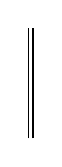
\begin{tikzpicture}\draw (0,0)--(0,1.4) (.06,0)--(.06,1.4);\end{tikzpicture}} à noter \unsure{comme|comme une|ce} propriété formelle \unsure{intéress.|intéressante}. \unsure{Cas contraire|Au contraire|Par contre} $\pm$ \unsure{génle.} \unsure{(au moins|(au voisin}, les \unsure{construction|contraires|conditions} \unsure{modérée|modérés}) des unions (cas non modéré) si $F$ et $G$ disjointes\ldots}
\inserted{\uline{Plus gén.}, ça marche pour Sup \unsure{quel.|quelc.} (au sens de $\leq$)}
En effet, on utilise le fait que les multistrates de $F\cup H$ sont les multistrates \deleted{qui sont communes à $F$} qui appartiennent à $F$, ou \deleted{à} $H$. Or la propriété de raffinement se vérifie sur les multistrates.

\uline{Définition} On dit alors que $F$ est une \inserted{\uline{subdivision}} de $G$.
